% body.tex
% 2024.02.20, by @zachleach

\setcounter{section}{3}

\subsection{Data rate}
\ii{It is desired to send a sequence of computer screen images over optical fiber. The screen is 3840 $\times$ 2160 pixels, each pixel being 24 bits. There are 60 screen images per second. What data rate is needed?}
\begin{align*}
	\text{Data Rate} = \frac{\text{Number of bits}}{\text{Bits per second}}
\end{align*}
%\vspace{4pt}

There are $24 \text{ bits} \cdot (3840 \times 2160)$ = 199,065,600 bits per image. Transmitting 60 images per second gives a data rate of data rate is $60 \cdot $ 199,065,600 = \ul{$1.194 \cdot 10^{10}$ bits per second.}

\subsection{Minimum bandwidth FDM}
\ii{Ten signals, each requiring 4000 Hz, are multiplexed onto a single channel using FDM. What is the minimum bandwidth required for the multiplexed channel? Assume that the guard bands are 400 Hz wide.}
% TODO fix this shit
\begin{align*}
	B = [c_n \cdot c_b] + [(c_n - 1) \cdot G_{\text{width}}]
	%\text{Bandwidth} = [\text{\# of channels} \cdot \text{channel bandwidth}] + [(\text{\# of channels} - 1) \cdot \text{guard band width}]
\end{align*}

Where $B$ represents the minimum bandwidth, $c_n$ represents the number of channels, $c_b$ represents the channel bandwidth, $G_{\text{width}}$ represents the guard band width. In this case, the minimum bandwidth required is $[10 \cdot 4000 \text{Hz}] + [(9) \cdot 400 \text{Hz}]$ = \ul{43,600 Hz.}

\subsection{Analog sampling}
\ii{A 3-kHz (analog) signal is sampled every 1 msec. What is the (minimum) data rate of a digital channel required to carry this signal? Assume that the quantization uses 256 levels.}
\begin{align*}
	\text{NEED TO FIX THIS}
	% \text{Minimum Data Rate} = 2 \times \text{Bandwidth} \times \log_2(\text{\# of Q-Levels})
\end{align*}
%\vspace{4pt}

The minimum data rate is $2 \times (3 \cdot 10^3) \times \log_2(256)$ = \ul{48,000 bits per second.}


\subsection{Network topologies}
\ii{Three packet-switching networks each contain n nodes. The first network has a star topology with a central switch, the second is a (bidirectional) ring, and the third is fully interconnected, with a wire from every node to every other node. What are the best-, average-, and worst-case transmission paths in hops?}

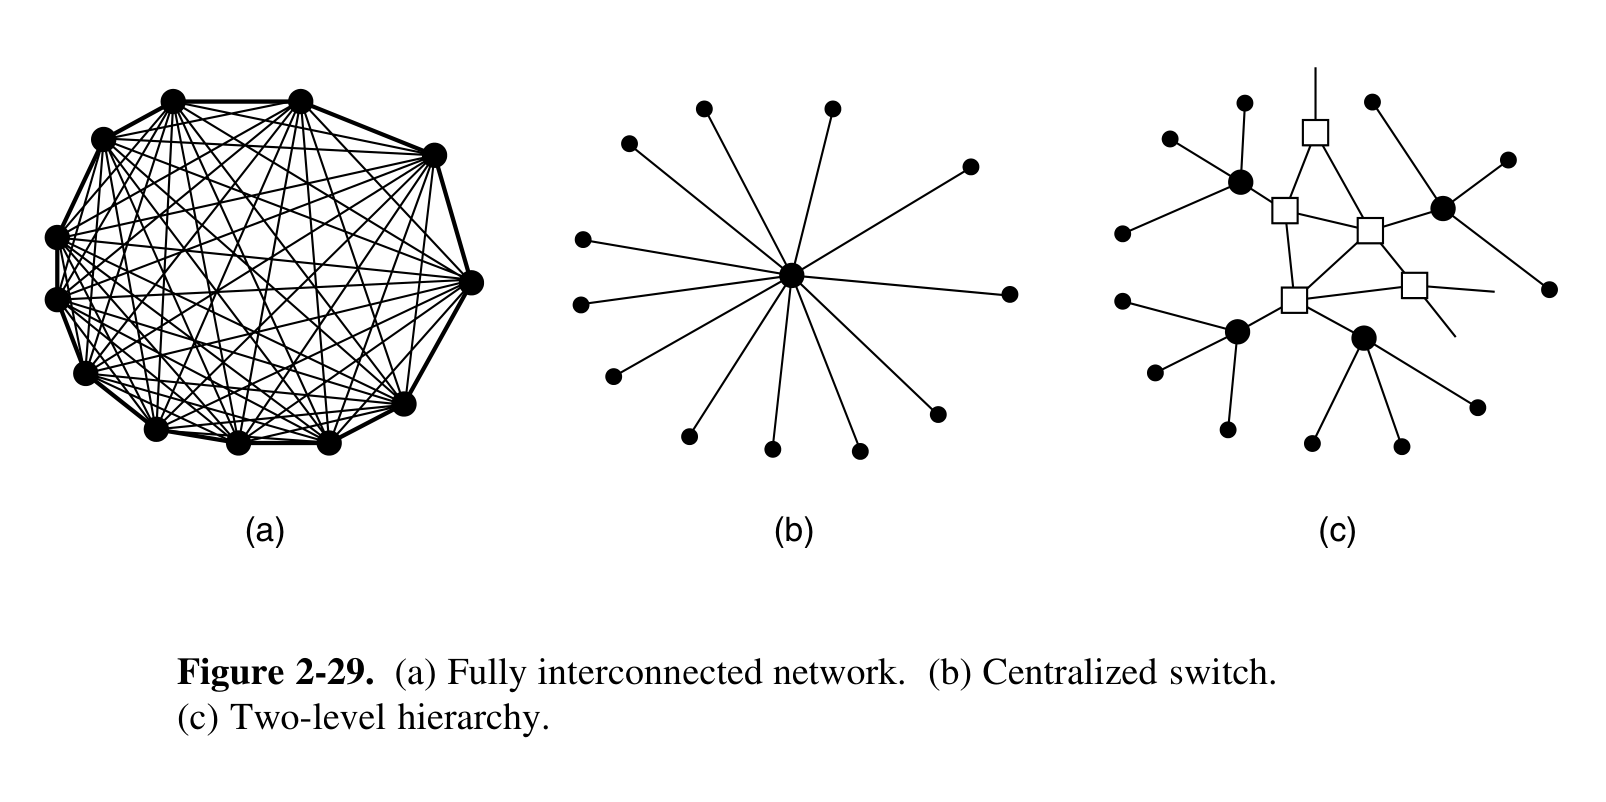
\includegraphics[width=\the\columnwidth]{network-topologies.png}

The best-, average-, and worst-case for \ul{star topology with central switch is 2 hops} (e.g., the hop from source to central switch, then from central switch to the destination).

The best-, average-, and worst-case for \ul{fully-interconnected network is 1 hop} (e.g., the hop from source to destination).

The best-, average-, and worst-case \ul{bi-directional ring is 1, $n / 2$, and $n - 1$ hops}, respectively (e.g., the source and destination nodes are adjacent, the average of 1 hop and $n - 1$ hops is $~ n/2$, and at worst the message must travel across all $n - 1$ nodes, respectively).

\subsection{Copper wire price}
\ii{A regional telephone company has 15 million subscribers. Each of their telephones is connected to a central office by a copper twisted pair. The average length of these twisted pairs is 10 km. How much is the copper in the local loops worth? Assume that the cross section of each strand is a circle 1 mm in diameter, the density of copper is 9.0 grams/cm3, and that copper sells for \$6 per kilogram.}
\begin{align*}
	V &= \pi \cdot r^2 \cdot h \\
	\text{Mass} &= \text{V} \cdot \text{Density} \\
	P &= \text{Mass} \cdot \text{Price per kg}
\end{align*}

The volume of the twisted pair is $\pi \cdot (0.05 \text{ cm})^2 \cdot $ (1,000,000 cm) = 7,854 cm $^3$. The mass is $9 \cdot (7,854)$ = 70,686 grams. The price is $6 \cdot (70.686)$ = \ul{\$424,115.}


\subsection{Downstream bandwidth}
\ii{A cable company decides to provide Internet access over cable in a neighborhood consisting of 5000 houses. The company uses a coaxial cable and spectrum allocation allowing 100 Mbps downstream bandwidth per cable. To attract customers, the company decides to guarantee at least 2 Mbps downstream bandwidth to each house at any time. Describe what the cable company needs to do to provide this guarantee.}
\begin{align*}
	B = H \cdot GB \\
\end{align*}

To guarantee 2 MBps downstream bandwidth to each of the 5,000 houses, the cable company will need to provide 5,000 $\cdot$ 2 Mbps = 10,000 Mbps total downstream bandwidth. Since the cable company has cables which can carry 100 Mbps, the cable company can use a multiplexing technique like FDM to divide the 10,000 Mbps into 100 cables each serving 50 houses.

\subsection{Sattelite Problem}
\ii{Calculate the end-to-end transit time for a packet for both GEO (altitude: 35,800 km), MEO (altitude: 18,000 km), and LEO (altitude: 750 km) satellites.}
\begin{align*}
	t = \frac{2 \cdot \Delta d}{c}
\end{align*}

For \ul{GEO: 0.233 seconds} [$2 \cdot (35,800) / 3\cdot 10^{5}$], \ul{MEO: 0.12 seconds} [$2 \cdot (18,000) / 3\cdot 10^5$], and \ul{LEO: 0.015 seconds} [$2 \cdot (750) / 3 \cdot 10^5$].




